
% xetex expected
\documentclass[xetex,professionalfont]{beamer}

% we want math
\usepackage{amsmath}

% fixes and extensions to amsmath
\usepackage{mathtools}

% additional math symbols
\usepackage{amssymb}

% good-looking fractions in text via \sfrac
\usepackage{xfrac}

% fix spaces after custom commands (see below for examples)
\usepackage{xspace}

% minted allows for fancy syntax highlighting (requires python with pygments)
% usage:
%   \begin{minted}{python}
%   codeb
%   \end{minted}
% \usepackage{minted}

% better looking tables
% usage:
%   begin with a \toprule, write a single row of column headings,
%   then add \midrule and after the columns of data we finish with \bottomrule
% example:
%   \begin{tabular}{llr} \toprule
%   Animal & Description & Price \midrule
%   cat & foo & 10 \\
%   dog & bar & 20 \\ \bottomrule
%   \end{tabular}
% note that good tables generally neither have vertical rules nor double rules
\usepackage{booktabs}

% system font support (requires xetex or luatex)
\usepackage{fontspec}
\setmonofont[Scale=0.7]{Cousine} % part of ttf-chromeos fonts on Arch

% improve microtypography
\usepackage{microtype}

% multi-language quotes for babel
\usepackage{csquotes}

% easy way to include copyright information
\usepackage{copyrightbox}

% better bibliographies
\usepackage[backend=biber,style=authoryear]{biblatex}

% language support (english,ngerman)
\usepackage[english]{babel}

% plots (part of texlive-pictures)
\usepackage{pgfplots}

% -----------------------------------------------------------------------------

% specify PDF metadata
\hypersetup{pdftitle={CVSP VO - 3D Vision},pdfsubject={},pdfauthor={Christopher Pramerdorfer}}

% copyright font style
\makeatletter\renewcommand{\CRB@setcopyrightfont}{\tiny\color{lightgray}}

% make emph bold
\DeclareTextFontCommand{\emph}{\bfseries}

% use tuwcvl beamer theme
\usetheme{tuwcvl}

% add bib file
\addbibresource{literature.bib}

% plot setup

\pgfplotsset{width=6.5cm,compat=1.11}

\definecolor{darkgreen}{rgb}{0,0.8,0.1}

% -----------------------------------------------------------------------------

% common english abbreviations
\newcommand{\ie}{\mbox{i.e.}\xspace} % i.e.
\newcommand{\eg}{\mbox{e.g.}\xspace} % e.g.
\newcommand{\wrt}{\mbox{wrt.}\xspace} % wrt.

% math - argmin and argmax
\DeclareMathOperator*{\argmin}{arg\,min}
\DeclareMathOperator*{\argmax}{arg\,max}

\DeclareMathOperator*{\Norm}{Norm}
\DeclareMathOperator*{\Uniform}{Uniform}
\DeclareMathOperator*{\Bern}{Bern}

% shortcuts for number ranges
\newcommand{\NN}{\mathbb{N}}
\newcommand{\ZZ}{\mathbb{Z}}
\newcommand{\QQ}{\mathbb{Q}}
\newcommand{\RR}{\mathbb{R}}

% bold vectors
\renewcommand{\vec}[1]{\ensuremath{\mathbf{#1}}}

% vector shortcuts
\newcommand{\va}{\vec{a}}
\newcommand{\vb}{\vec{b}}
\newcommand{\vc}{\vec{c}}
\newcommand{\ve}{\vec{e}}
\newcommand{\vr}{\vec{r}}
\newcommand{\vs}{\vec{s}}
\newcommand{\vt}{\vec{t}}
\newcommand{\vu}{\vec{u}}
\newcommand{\vv}{\vec{v}}
\newcommand{\vw}{\vec{w}}
\newcommand{\vx}{\vec{x}}
\newcommand{\vy}{\vec{y}}
\newcommand{\vz}{\vec{z}}

% bold greek symbols
\newcommand{\bth}{\boldsymbol{\theta}}
\newcommand{\intr}{\boldsymbol{\Lambda}}

% -----------------------------------------------------------------------------

\title{Computer Vision Systems Programming VO}
\subtitle{3D Vision}
\author{Christopher Pramerdorfer}
\institute{Computer Vision Lab, Vienna University of Technology}

\begin{document}

% -----------------------------------------------------------------------------

\begin{frame}
\maketitle
\end{frame}

% -----------------------------------------------------------------------------

\begin{frame}
\frametitle{Topics}

Image formation\\\medskip
3D data acquisition

\bigskip
\begin{center}
    \copyrightbox[b]
    {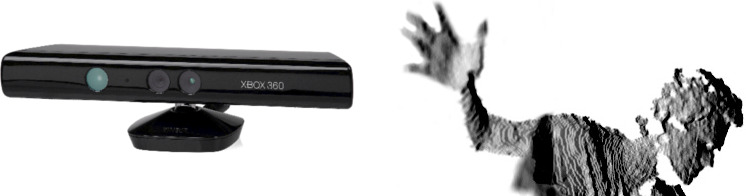
\includegraphics[width=10cm]{figures/intro-collage.jpg}}
    {\centering Images from \url{wikipedia.org}, \url{createiveapplications.net}}
\end{center}

\end{frame}

% -----------------------------------------------------------------------------

\begin{frame}
\frametitle{Motivation}

Many CV applications rely on knowledge of scene geometry

\bigskip
This lecture covers
\begin{itemize}
    \item How scene geometry and images are related
    \item How this relation can be used to recover scene geometry % that is different means for obtaining an estimation of the scene geometry from images
\end{itemize}

\end{frame}

% -----------------------------------------------------------------------------

\begin{frame}
\frametitle{Image Formation}
\framesubtitle{Pinhole Camera Model}

\bigskip
\begin{center}
    \copyrightbox[b]
    {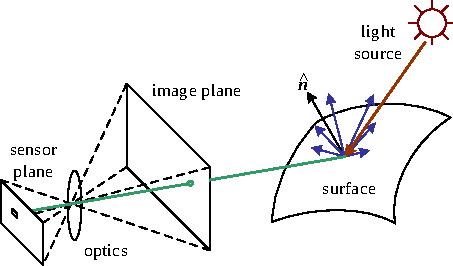
\includegraphics[width=7cm]{figures/image-formation.pdf}} % the pinhole camera model usually places the image plane in front of the pinhole for convenience, even though that's not physically possible.
    {\centering Image from \cite{szeliski2010}}
\end{center}

\end{frame}

% -----------------------------------------------------------------------------

\begin{frame}
\frametitle{Image Formation}
\framesubtitle{Pinhole Camera Model}

\bigskip
\begin{center}
    \copyrightbox[b]
    {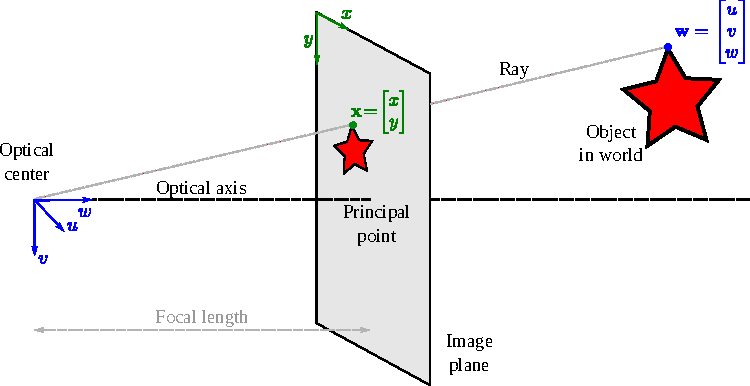
\includegraphics[width=9cm]{figures/pinhole-model.pdf}} % the model in the image is simplified in the sense that the camera is centered at the origin of the world coordinate system and because there is no skew
    {\centering Image adapted from \cite{prince12}}
\end{center}

\end{frame}

% -----------------------------------------------------------------------------

\begin{frame}
\frametitle{Image Formation}
\framesubtitle{Pinhole Camera Model}

We obtain $x=fu/w+p_x$, $y=fv/w+p_y$ % here we disregard the skew parameter, which is fine with modern cams
\begin{itemize}
    \item $f$ : focal length in pixels % we have a digital camera, so f is measured in pixels. also, in general it is possible that f differs along x and y due to the spacing of receptor cells, but with modern cams this is usually not the case
    \item $p_x,p_y$ : image coordinates of the principal point % this usually is half the image resolution because the sensor is centered at the optical center, as in the previous image
\end{itemize}

\bigskip
This mapping is linear in \emph{homogeneous coordinates} % therefore geometric problems are usually solved in homogeneous coordinates, for example to estimate an initial solution (see Prince's book for examples) (it is not linear above because of the division by w)
\begin{eqnarray*}
    \lambda
    \tilde{\vx} &=& % we use tilde for homogeneous coordinates with the last one being 1
    \begin{pmatrix}
         \intr & \vec{0} % the left 3x3 matrix below captures the intrinsic camera parameters, that is the relation between image and world coordinates if the center of projection coincides with the world coordinate system (i.e. if the world and camera coordinate systems are equal)
     \end{pmatrix} \tilde{\vw} \\
     \lambda
    \begin{pmatrix}
        x \\ y \\ 1
    \end{pmatrix} &=& 
    \begin{pmatrix}
        f & 0 & p_x & 0 \\ 0 & f & p_y & 0 \\ 0 & 0 & 1 & 0
    \end{pmatrix}
    \begin{pmatrix}
        u \\ v \\ w \\ 1
    \end{pmatrix}
\end{eqnarray*} % these equations are "exact", but in practice we have to round at some point because the sensor is comprised of individual sensor cells

\end{frame}

% -----------------------------------------------------------------------------

\begin{frame}
\frametitle{Image Formation}
\framesubtitle{Pinhole Camera Model}

World and camera coordinate systems generally differ
\begin{itemize}
    \item Transform $\vw$ to camera coordinates before projection
\end{itemize}
\begin{eqnarray*}
    \vw' &=& \boldsymbol{\Omega}\vw + \boldsymbol{\tau} \\
    \begin{pmatrix}
        u' \\ v' \\ w'
    \end{pmatrix} &=&
    \begin{pmatrix}
        \omega_{11} & \omega_{12} & \omega_{13} \\
        \omega_{21} & \omega_{22} & \omega_{23} \\
        \omega_{31} & \omega_{32} & \omega_{33} \\
    \end{pmatrix}
    \begin{pmatrix}
        u \\ v \\ w
    \end{pmatrix} +
    \begin{pmatrix}
        \tau_u \\ \tau_v \\ \tau_w
    \end{pmatrix}
\end{eqnarray*}

\end{frame}

% -----------------------------------------------------------------------------

\begin{frame}
\frametitle{Image Formation}
\framesubtitle{Pinhole Camera Model}

We obtain the full \emph{pinhole camera model}
\[\lambda\tilde{\vx}=\begin{pmatrix}
    \intr & \vec{0}
\end{pmatrix}
\begin{pmatrix}
    \boldsymbol{\Omega} & \boldsymbol{\tau} \\ \vec{0}^\top & 1
\end{pmatrix}\tilde{\vw}\]
% the combination of the intrinsic and extrinsic matrices is called the camera matrix. note that this matrix is 3x4. if we want to inverse the process we need the inverse camera matrix, which only exists for square matrices, so we append a (0 0 0 1) row to the intrinsics matrix to achieve this

\bigskip
Standard camera model in CV
\begin{itemize}
    \item Usually together with radial distortion correction % while most inaccuracies due to the approximative model can usually be disregarded, radial distortions can be so severe (depending on the lens) that they must be corrected
\end{itemize}

\bigskip
Approximation to actual image formation
\begin{itemize}
    \item In practice $\vw$ is not mapped to a single $\vx$ % because of lens distortions, as covered in several other lectures
\end{itemize}

\end{frame}

% -----------------------------------------------------------------------------

\begin{frame}
\frametitle{Computing Scene Geometry}

We can obtain $\vw$ by inverting the pinhole camera model % respectively the 4x4 camera matrix, see above
\begin{itemize}
    \item But we don't know $w$ % see the above figure ... w = lambda is lost during perspective projection ... in normalized coodinates ("no" extrinsics, px=py=0, f=1), lambda*~x in the above equation corresponds to the ray that intersects both x (at lambda=1), w (at lambda=w), and the optical center (at lambda=0) ... if we dont know lambda, we dont know "where to stop"
\end{itemize}

\bigskip
To this end, we must
\begin{itemize}
    \item Utilize information from multiple images % of the same scene
    \item Use sensors that capture $w$ directly
\end{itemize}

% note that this is not exhaustive. for example there are methods that can be used if we know the reflectance properties of the objects we observe, and if the scene is planar we can reconstruct it as well ... here we talk about means that work in general, without knowledge of the scene

\end{frame}

% -----------------------------------------------------------------------------

\begin{frame}
\frametitle{Computing Scene Geometry}
\framesubtitle{Stereo}

\begin{center}
    \copyrightbox[b]
    {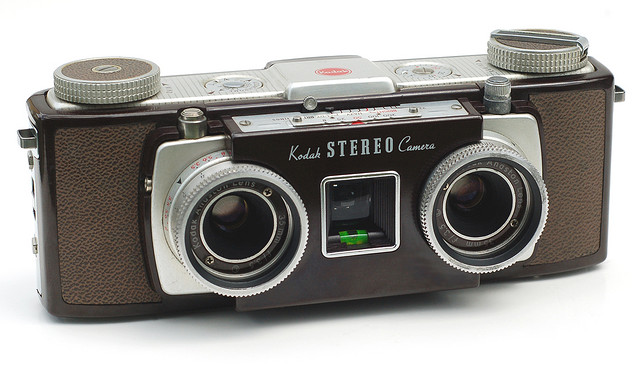
\includegraphics[width=6.5cm]{figures/kodak-stereo.jpg}}
    {\centering Image by John Kratz / flickr}
\end{center}

\end{frame}

% -----------------------------------------------------------------------------

\begin{frame}
\frametitle{Computing Scene Geometry}
\framesubtitle{Stereo}

In \emph{stereo reconstruction} we have
\begin{itemize}
    \item Point correspondences $\{(\vx_1,\vx_2)\}$ in two images % works also with multiple cameras of course
    \item Taken with calibrated cameras (known $\intr, \boldsymbol{\Omega}, \boldsymbol{\tau}$)
\end{itemize}

\bigskip
Goal is to estimate corresponding world coordinates $\vw$
\begin{itemize}
    \item Accomplished via triangulation % we know the two rays on which the point must lie. since both x1 and x2 are projections of the same point, the corresponding rays intersect at some point, namely at w
\end{itemize}

\end{frame}

% -----------------------------------------------------------------------------

\begin{frame}
\frametitle{Computing Scene Geometry}
\framesubtitle{Stereo}

\begin{center}
    \copyrightbox[b]
    {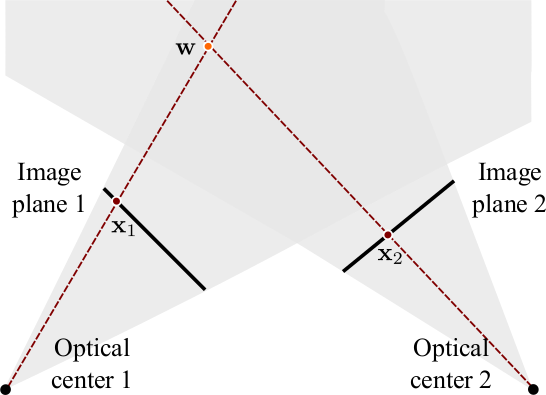
\includegraphics[width=6cm]{figures/triangulation.png}}
    {\centering Image from \cite{prince12}}
\end{center}

\end{frame}

% -----------------------------------------------------------------------------

\begin{frame}
\frametitle{Computing Scene Geometry}
\framesubtitle{Stereo}

The challenge is finding correspondences

\bigskip
We typically want
\begin{itemize}
    \item Many correspondences % so that we get a dense 3d reconstruction
    \item High accuracy and low noise
\end{itemize}

\bigskip
Usually accomplished via
\begin{itemize}
    \item Dense feature matching along epipolar lines
    \item Followed by local or global optimization % here we basically enforce that adjacent pixels have similar w, that is some form of regularization. see next slides
\end{itemize}

\end{frame}

% -----------------------------------------------------------------------------

\begin{frame}
\frametitle{Computing Scene Geometry}
\framesubtitle{Stereo}

$\vx_1$ must lie on the \emph{epipolar line} % this significantly reduces the complexity
\begin{itemize}
    \item Given by $\vx_0$ and the camera parameters % relation between the cameras, see below commend
\end{itemize}

\begin{center}
    \copyrightbox[b]
    {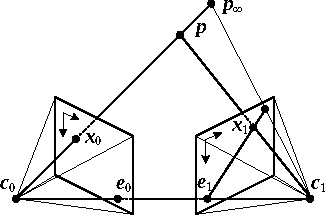
\includegraphics[width=6cm]{figures/epipolar-geometry.pdf}} % if we have two calibrated cameras, the point x1 that corresponds to x0 must lie on the epipolar line that is given by the essential matrix E, ~x1*E*~x0=0 ... ee Szeliski's book
    {\centering Image from \cite{szeliski2010}}
\end{center}

\end{frame}

% -----------------------------------------------------------------------------

\begin{frame}
\frametitle{Computing Scene Geometry}
\framesubtitle{Stereo}

Images are \emph{rectified} before correspondence search % this transforms the images so that x0 and x1 lie on the same scanline in both images, which facilitates the correspondence search
\begin{itemize}
    \item Relation between $x$-offset (\emph{disparity} $d$) and $w$, $d=fb/w$ % f is again the focal length in pixels
    \item $b$ is the distance between the cameras % along u because the cams are aligned (see below)
\end{itemize}

% rectification transforms the image pair as if it was captures with only an offset along u (as shown in the Kodak camera image above)

\bigskip
\begin{center}
    \copyrightbox[b]
    {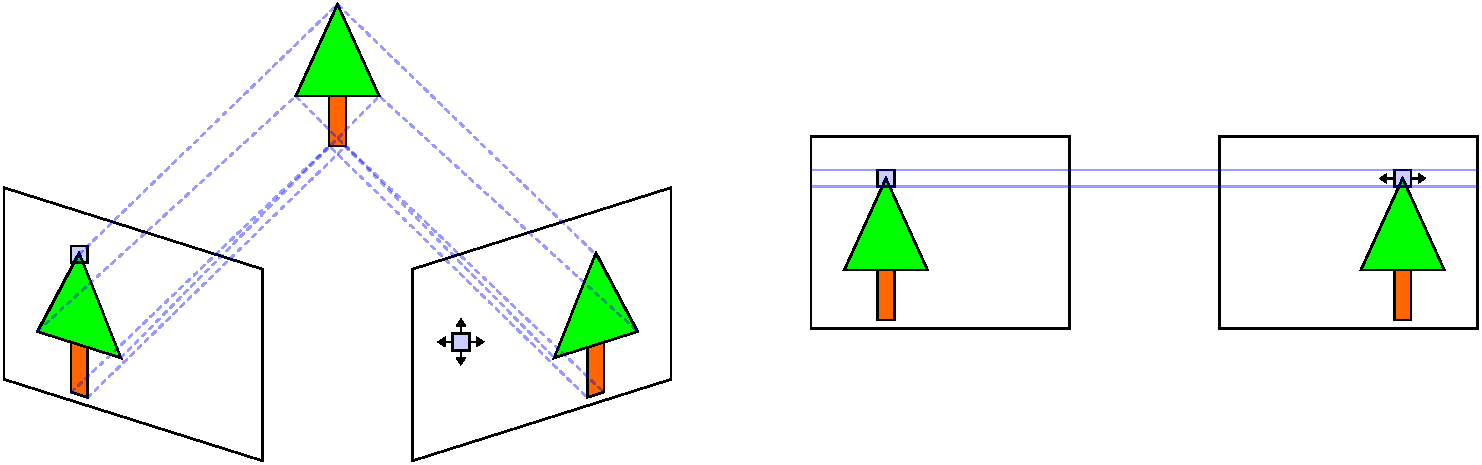
\includegraphics[width=10cm]{figures/rectification.pdf}}
    {\centering Image adapted from \url{wikipedia.org}}
\end{center}

\end{frame}

% -----------------------------------------------------------------------------

\begin{frame}
\frametitle{Computing Scene Geometry}
\framesubtitle{Stereo}

Dense matching on rectified images results in a \emph{disparity map}

\bigskip
\begin{center}
    \copyrightbox[b]
    {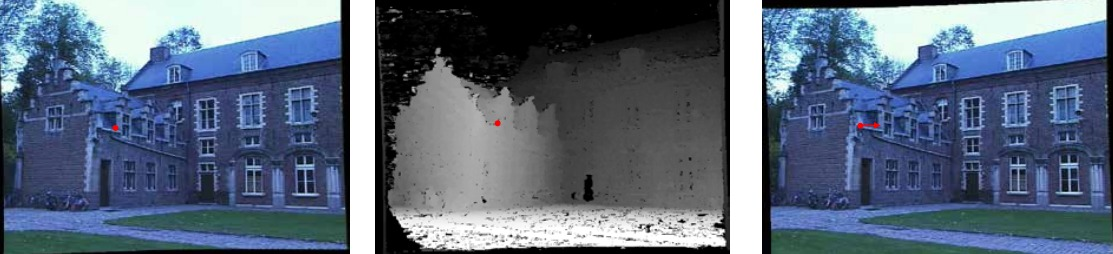
\includegraphics[width=10cm]{figures/rectified-stereo.jpg}} % we see that the result is quite noisy
    {\centering Image from Guido Gerig's slides}
\end{center}

\end{frame}

% -----------------------------------------------------------------------------

\begin{frame}
\frametitle{Computing Scene Geometry}
\framesubtitle{Stereo}

Raw disparity maps are noisy\\\medskip
Quality can be improved by encouraging smoothness\\\medskip
Accomplished via graphical models (\eg MRFs) % we always talk about models, which we've introduced earlier. see Prince for more information

\bigskip
\begin{center}
    \copyrightbox[b]
    {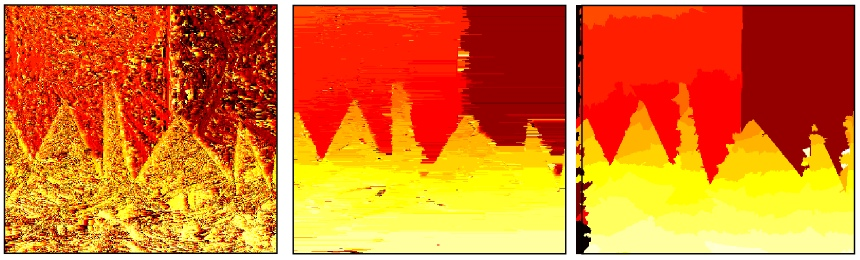
\includegraphics[width=10cm]{figures/dense-stereo-models.jpg}}
    {\centering Images from \cite{prince12}}
\end{center}

\end{frame}

% -----------------------------------------------------------------------------

\begin{frame}
\frametitle{Computing Scene Geometry}
\framesubtitle{Depth Sensors}

Alternatively, we can use sensors that capture $w$ directly
\begin{itemize}
    \item Usually together with brightness or color
\end{itemize}

\bigskip
These \emph{depth sensors}
\begin{itemize}
    \item Do not rely on texture
    \item Work under dim or dark conditions
    \item Save computational resources % because they to stereo matching on the sensor
\end{itemize}

\end{frame}

% -----------------------------------------------------------------------------

\begin{frame}
\frametitle{Computing Scene Geometry}
\framesubtitle{Depth Sensors -- Kinect v1}

Released by Microsoft for Xbox 360 in late 2010\\\medskip
Fastest selling consumer electronics device to date % according to http://www.guinnessworldrecords.com/records-9000/fastest-selling-gaming-peripheral/

\bigskip
\begin{center}
    \copyrightbox[b]
    {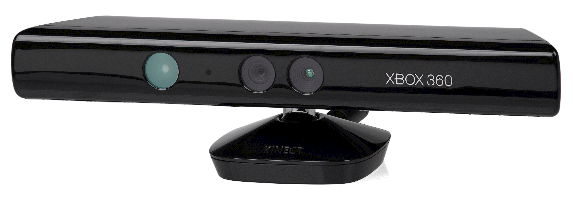
\includegraphics[width=7cm]{figures/kinect.png}}
    {\centering Image from \url{wikipedia.org}}
\end{center}

\end{frame}

% -----------------------------------------------------------------------------

\begin{frame}
\frametitle{Computing Scene Geometry}
\framesubtitle{Depth Sensors -- Kinect v1}

Works by replacing one sensor with an IR source
\begin{itemize}
    \item Projects a speckle pattern onto objects \url{https://www.youtube.com/watch?v=t5joFtzEYpo}
\end{itemize}

\bigskip
Pattern is observed using an IR sensor 

\bigskip
Stereo (epipolar) geometry still applies % we now just project light, not measure it, but we still have a rectified stereo pair (look at the image of the sensor)
\begin{itemize}
    \item Shift between patterns corresponds to $d$ respectively $w$ % shift between projected and observed pattern
\end{itemize}

\bigskip
Does not work in sunlight due to IR radiation % i.e. indoor only!

\end{frame}

% -----------------------------------------------------------------------------

\begin{frame}
\frametitle{Computing Scene Geometry}
\framesubtitle{Depth Sensors -- Kinect v1}

\begin{center}
    \copyrightbox[b]
    {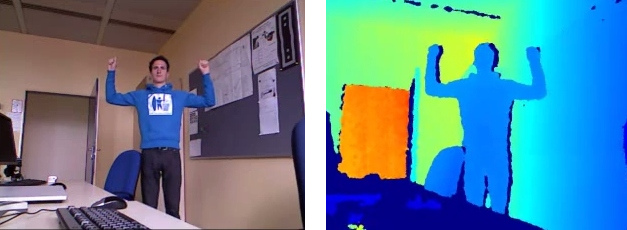
\includegraphics[width=10cm]{figures/kinect-matlab-screenshot.jpg}}
    {\centering Image from \url{https://www.youtube.com/watch?v=oOCMr0D7BqY}}
\end{center}

\end{frame}

% -----------------------------------------------------------------------------

\begin{frame}
\frametitle{Computing Scene Geometry}
\framesubtitle{Depth Sensors -- Kinect v2}

Released by Microsoft in late 2013

\begin{center}
    \copyrightbox[b]
    {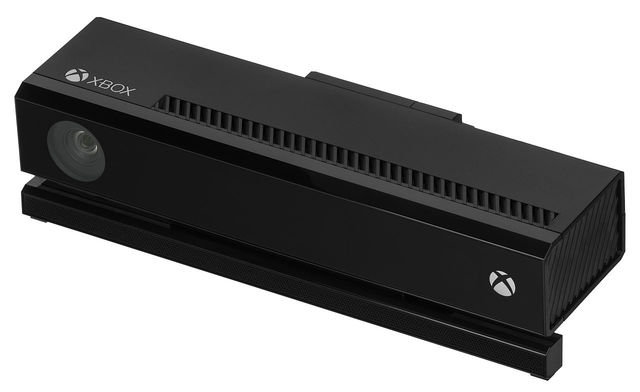
\includegraphics[width=7cm]{figures/kinect2.jpg}}
    {\centering Image from \url{wikipedia.org}}
\end{center}

\end{frame}

% -----------------------------------------------------------------------------

\begin{frame}
\frametitle{Computing Scene Geometry}
\framesubtitle{Depth Sensors -- Kinect v2}

Works based on the time of flight principle
\begin{itemize}
    \item A light pulse is emitted at time $t_0$
    \item Pulse is reflected and observed at time $t_1$
    \item $w$ proportional to delay, $t_1-t_0=2w/c$ % c is the speed of light
\end{itemize}

% Kinect2 seems to use a pulsed/gated design according to http://www.gamasutra.com/blogs/DanielLau/20131127/205820/The_Science_Behind_Kinects_or_Kinect_10_versus_20.php , but I could not find official information

\end{frame}

% -----------------------------------------------------------------------------

\begin{frame}
\frametitle{Computing Scene Geometry}
\framesubtitle{Depth Sensors -- Kinect v2}

\begin{center}
    \copyrightbox[b]
    {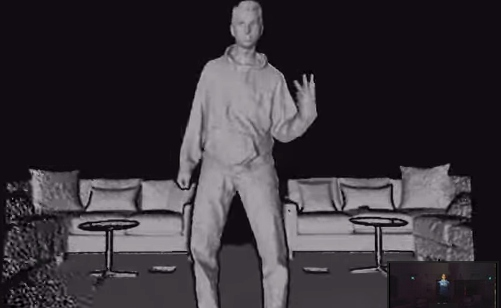
\includegraphics[width=7cm]{figures/kinect2-depth.jpg}}
    {\centering Image from \url{https://www.youtube.com/watch?v=JaOlUa57BWs}}
\end{center}

\end{frame}

% -----------------------------------------------------------------------------

\begin{frame}
\frametitle{Computing Scene Geometry}

We now have an image encoding $w$ (\emph{depth map})
\begin{itemize}
    \item Can be generated from disparity map as shown above
\end{itemize}

\bigskip
We can use this information to obtain points in the world $\vw$
\begin{itemize}
    \item By inverting the pinhole camera model
    \item Resulting in a \emph{point cloud}
\end{itemize}

\end{frame}

% -----------------------------------------------------------------------------

\begin{frame}
\frametitle{Computing Scene Geometry}

\begin{center}
    \copyrightbox[b]
    {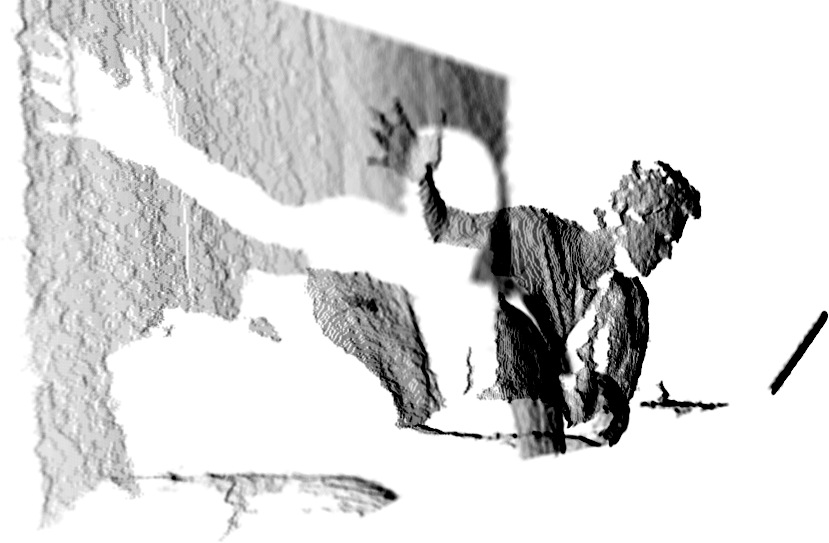
\includegraphics[width=8cm]{figures/point-cloud.jpg}}
    {\centering Image from \url{creativeapplications.net}}
\end{center}

\end{frame}

% -----------------------------------------------------------------------------

\begin{frame}
\frametitle{Summary}

We have covered
\begin{itemize}
    \item How the scene geometry and images are related
    \item Means for estimating point distances $w$
    \item How scene geometry can be recovered on this basis
\end{itemize}

\bigskip
This information enables interesting CV applications
\begin{itemize}
    \item Next, we will go over some examples
\end{itemize}

\end{frame}

% -----------------------------------------------------------------------------

\begin{frame}
\frametitle{3D Vision Lecture}

Interested in 3D vision?
\begin{itemize}
    \item There is an own VO (183.129) and UE (183.130)
\end{itemize}

\end{frame}

% -----------------------------------------------------------------------------

\begin{frame}
\frametitle{Bibliography}

\printbibliography

\end{frame}

\end{document}
